
\documentclass[conference]{IEEEtran}
\usepackage{amsmath,amsfonts}
\usepackage{algorithmic}
\usepackage{algorithm}
\usepackage{array}
\usepackage[caption=false,font=normalsize,labelfont=sf,textfont=sf]{subfig}
\usepackage{textcomp}
\usepackage{stfloats}
\usepackage{url}
\usepackage{verbatim}
\usepackage{graphicx}
\usepackage{cite}
\usepackage{pdfpages}
\usepackage{booktabs}
\usepackage{hyperref}

\usepackage[skip=6pt]{caption}

\begin{document}

\title{Classificazione Binaria del Diabete}

\author{
\IEEEauthorblockN{Chiodo Martina}
\IEEEauthorblockA{Matricola: s343310 }
\and
\IEEEauthorblockN{Danca Ema-Aldona}
\IEEEauthorblockA{Matricola: s347940 }
\and
\IEEEauthorblockN{Speca Leonardo}
\IEEEauthorblockA{Matricola: s343483 }
\and
\IEEEauthorblockN{Terenziani Andrea}
\IEEEauthorblockA{Matricola: s349167}
\and
\IEEEauthorblockN{Vigè Sophie}
\IEEEauthorblockA{Matricola: s339268 }
}

\maketitle

\begin{abstract}
%L'abstract serve a riassumere brevemente quello che presenta il report. Per istruzioni dettagliate sul formato fare riferimento al file ``New\_IEEEtran\_how-to.tex''.
Il report descrive il processo di selezione, addestramento e validazione di alcuni algoritmi di classificazione binaria implementati in Python facendo largo uso della libreria Scikit-Learn.
In particolare, vengono analizzati l’approccio adottato, le caratteristiche del dataset utilizzato, il preprocessing e l’efficacia degli algoritmi proposti nel distinguere correttamente tra pazienti diabetici e non diabetici.
\end{abstract}

\section{Introduzione}

Una delle sfide del settore sanitario è la diagnosi precoce delle malattie croniche che richiede un continuo miglioramento degli strumenti diagnostici. Una di queste è la classificazione accurata dei pazienti affetti da diabete. %Individuare il diabete in fase precoce è difficile a causa dei numerosi fattori di rischio coinvolti e delle differenze tra un paziente e l’altro.\\

La diagnosi viene tradizionalmente effettuata grazie alla valutazione del personale medico degli esami clinici. Tuttavia, questo metodo può risultare lento, soggettivo e difficile da applicare su larga scala. Inoltre, l’analisi manuale di grandi volumi di dati clinici può essere onerosa sia in termini di tempo che di risorse economiche. 
%Per rispondere a questa esigenza, è stato sviluppato un sistema automatico di classificazione dei pazienti affetti da diabete. 
In questa ricerca, abbiamo utilizzato diversi algoritmi di classificazione binaria basati su alcune caratteristiche dei pazienti.
%, come il sesso, l’età, la presenza di ipertensione o malattie cardiache, la storia del fumo, l’indice di massa corporea, i livelli di emoglobina glicata e di glucosio nel sangue, e altri indicatori biologici.



\section{Analisi dei dati}
%Caratterizzare i dati tramite grafici e descrizione testuale.
Il materiale fornito è comprensivo di due dataset, uno per la fase di training e uno per quella di test. Questi presentano informazioni cliniche e demografiche raccolte su pazienti con e senza diabete. Il dataset di training è composto da 588 record, di cui solo un quarto di questi rappresenta pazienti con il diabete. Le variabili considerate includono fattori quali sesso, età, ipertensione, malattie cardiache, abitudini legate al fumo, indice di massa corporea (BMI), livello di emoglobina glicata (HbA1c), livello di glucosio nel sangue, sensibilità all’insulina, interazione tra BMI e glucosio e presenza di Troponina T. 

\begin{figure}[htbp]
    \centering
    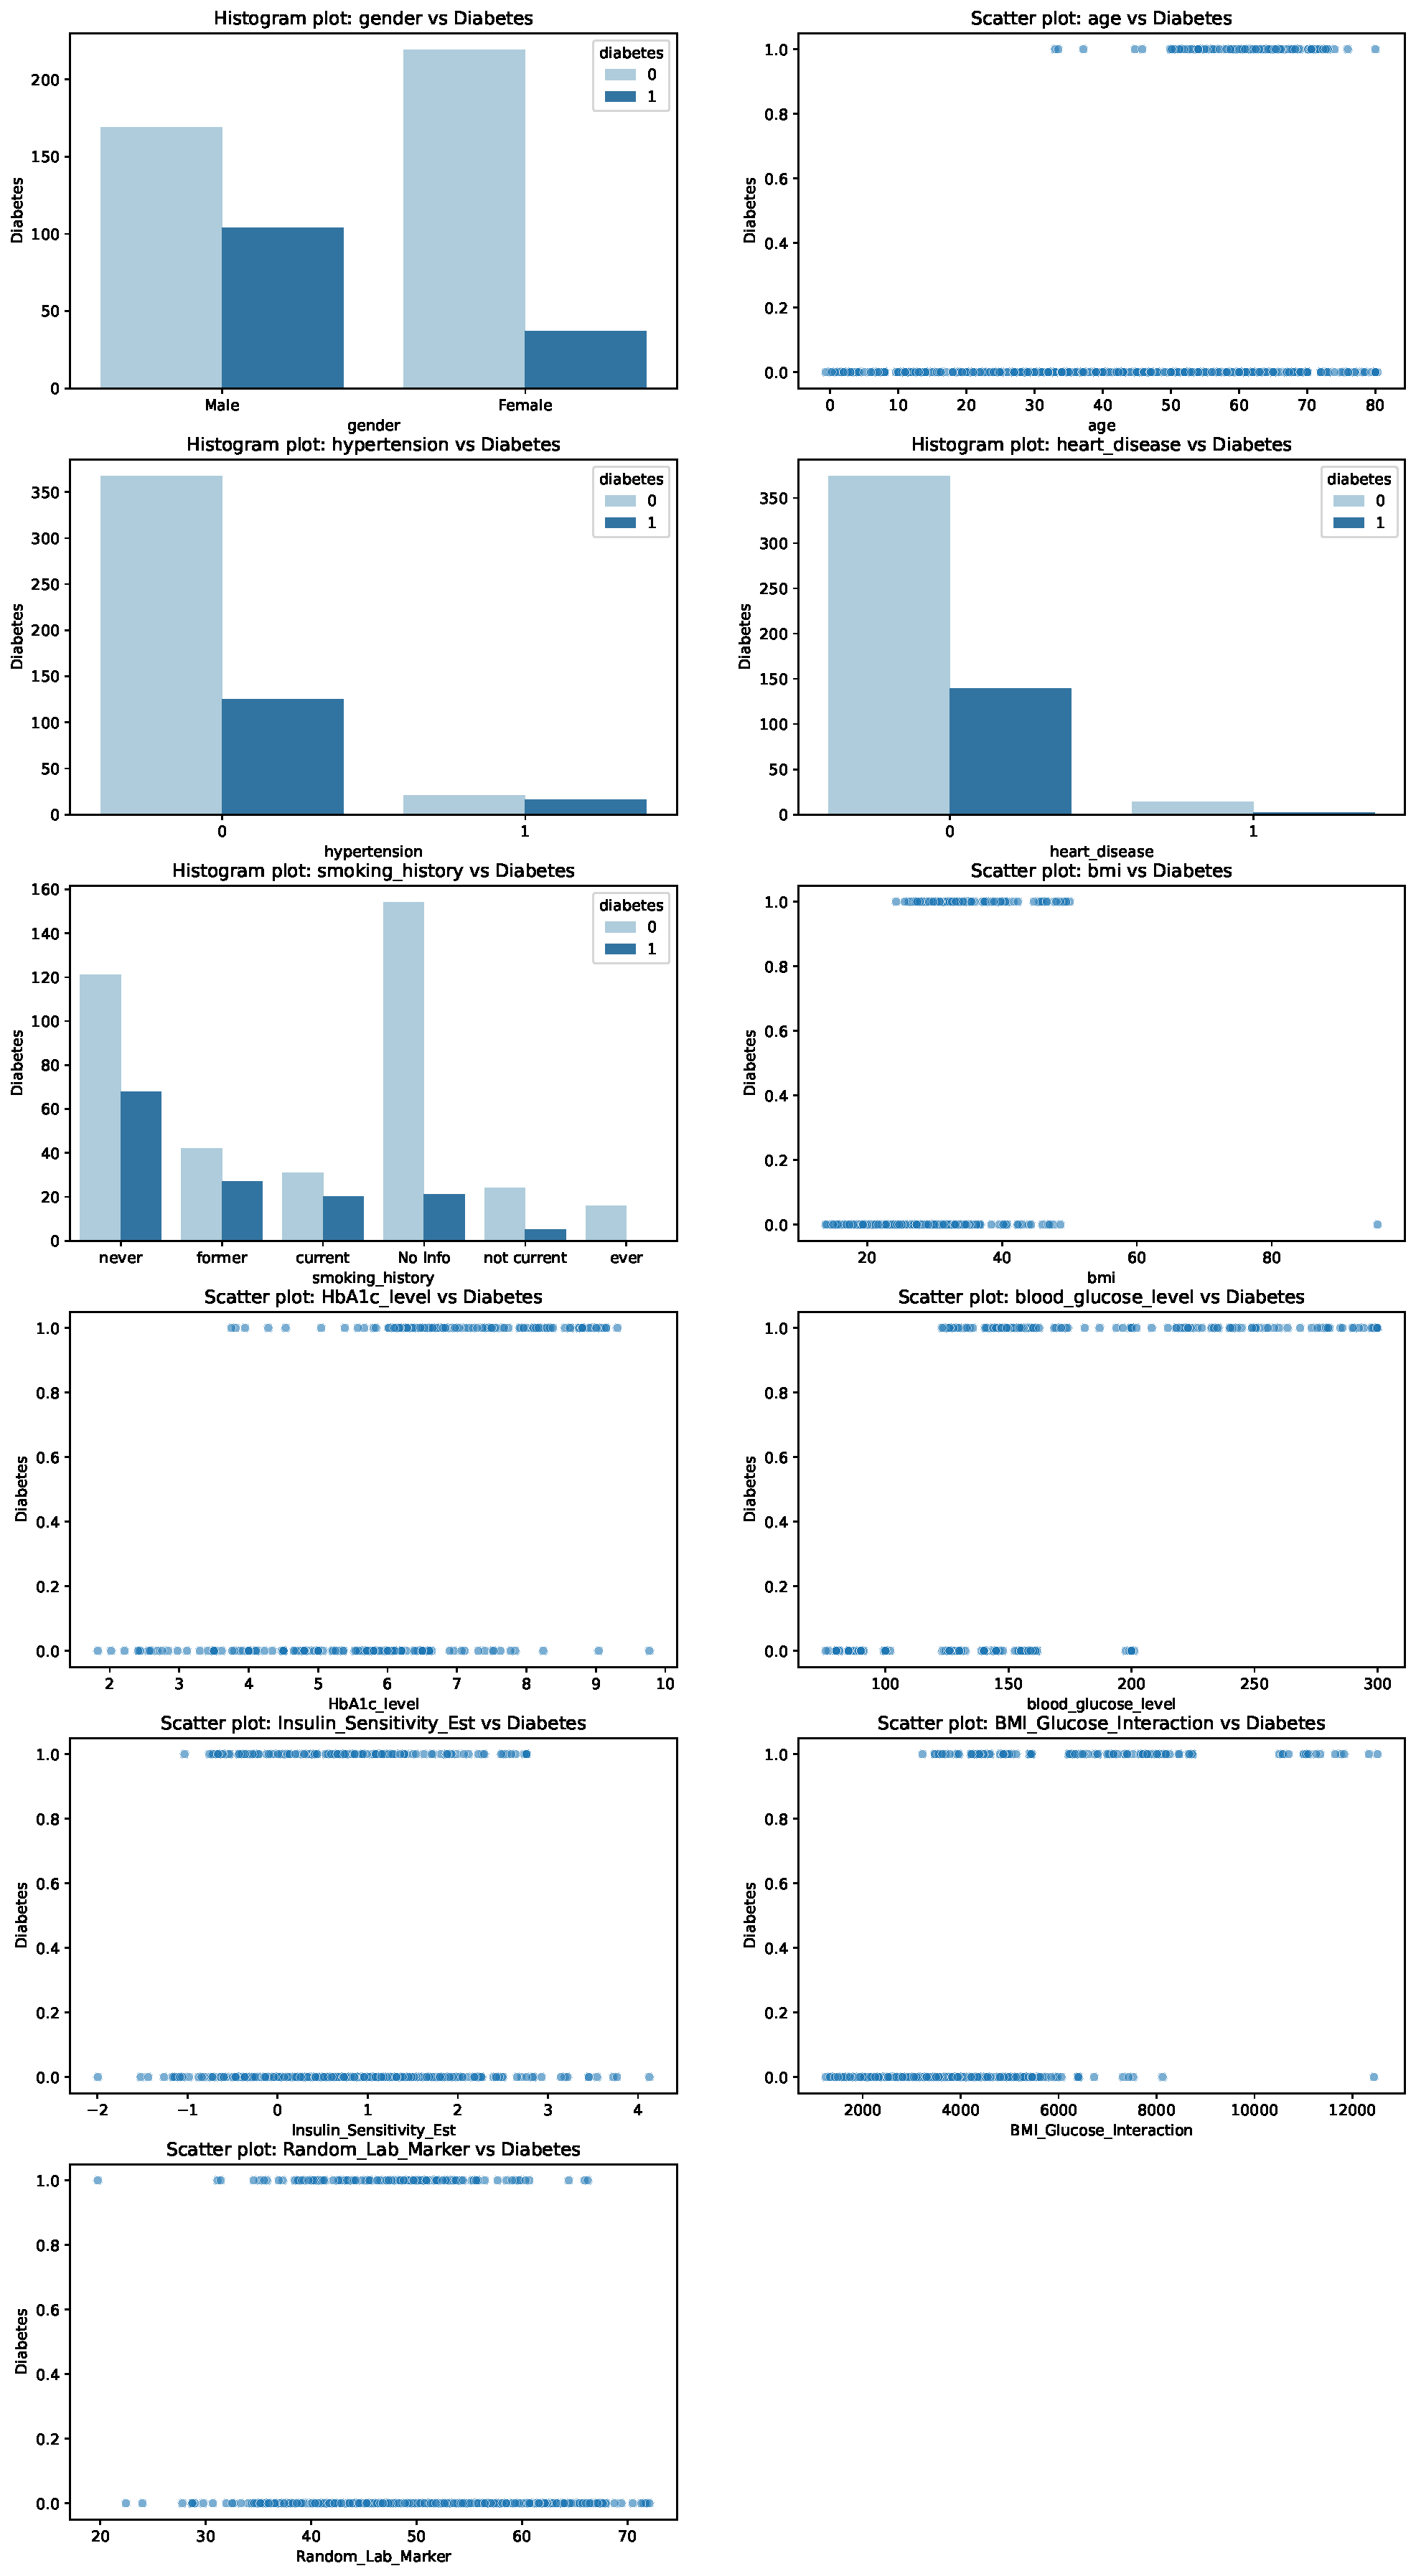
\includegraphics[width=0.43\textwidth]{features_vs_diabetes.pdf}
    \caption{Scatter plot di ogni feature e della variabile risposta}
    \label{features}
\end{figure}

I dati sono stati sottoposti a una fase preliminare di pre-elaborazione per garantirne la qualità e l’affidabilità.

Un'analisi esplorativa iniziale ha rilevato 59 record duplicati nel train set, successivamente rimossi. L’attributo \emph{smoking\_history} conteneva la voce “No Info”, trattata come categoria a sé stante per evitare la perdita di dati, data la dimensione già ridotta del dataset. Poiché la variabile assume solo 6 valori categorici, a nostro avviso, ordinabili, si è optato per una codifica manuale invece del one-hot encoding, con il seguente ordine: “never”, “ever”, “No Info”, “not current”, “former”, “current”. Anche l’attributo \emph{gender} è stato codificato, in questo caso tramite \texttt{LabelEncoding}.

Per quanto riguarda invece i valori mancanti dell'attributo \emph{Insulin\_Sensitivity\_Est} si è deciso di utilizzare il valore medio in quanto (dai grafici esplorativi che seguono) non sembra che tale attributo abbia una forte correlazione con la variabile risposta. 
Questo è stato fatto usando la trasformazione \texttt{SimpleImputer(strategy='mean')}, la quale è stata fittata sui dati di train e poi usata per trasformare sia il train che il test set.

Successivamente, si è voluto indagare sulla presenza di outlier, ovvero valori anomali che si discostano significativamente dalla distribuzione dei dati, per cui si è proceduto con tecniche di pulizia dei dati. A tale scopo sono stati imposti alcuni vincoli di dominio sulle feature, i quali hanno portato all'eliminazione dei record con età negativa o BMI negativo o superiore a 90 ad esempio (outlier che erano presenti nei dataset come mostrano i grafici \ref{features} e \ref{hist}). 

Infine, per garantire un’elaborazione adeguata dei dati e l’utilizzo corretto degli algoritmi, senza dare pesi diversi agli attributi numerici sulla base del loro range di valori, i valori di tutti gli attributi (meno l'attributo \emph{Insulinity\_Sensitivity\_Est} poiché è già frutto di una normalizzazione) sono stati riscalati tramite \texttt{MinMAxScaler()} nell'intervallo $\left[ -3;3\right]$. Si è scelto questo intervallo poiché è il range di dominio dell'attributo \emph{Insulinity\_Sensitivity\_Est}.

La Figura \ref{features} offre un’analisi qualitativa delle feature più influenti sulla classificazione, mostrando la relazione tra ciascuna e la variabile target. Ad esempio, valori elevati di \emph{Blood\_Glucose\_Level} e \emph{HbA1c\_level} sono frequentemente associati a casi positivi di diabete, mentre \emph{Insulin\_Sensitivity\_Est} mostra una correlazione meno evidente. Tra le variabili categoriche, si osserva che i pazienti di sesso maschile e quelli con una storia di fumo "former" o "current" risultano più inclini a sviluppare il diabete rispetto alle altre classi.


Si è poi fatto un lavoro di feature selection basata sulla matrice di correlazione (Figura \ref{correlation}). Questa evidenzia una correlazione molto alta tra l'attributo \emph{BMI\_Glucose\_Interaction} e gli attributi \emph{bmi} e \emph{blood\_glucose\_level}, come era prevedibile dal nome. Si è quindi deciso di eliminare la feature di interazione perché, sebbene abbia una correlazione alta con la risposta binaria, questa dipendenza viene spiegata dagli altri due attributi. Le feature con bassa correlazione rispetto alla variabile target sono state mantenute, sia per la presenza di meccanismi interni di selezione nei modelli utilizzati, sia perché la ridotta dimensionalità del dataset non giustificava ulteriori eliminazioni.

\begin{figure}[htbp]
    \centering
    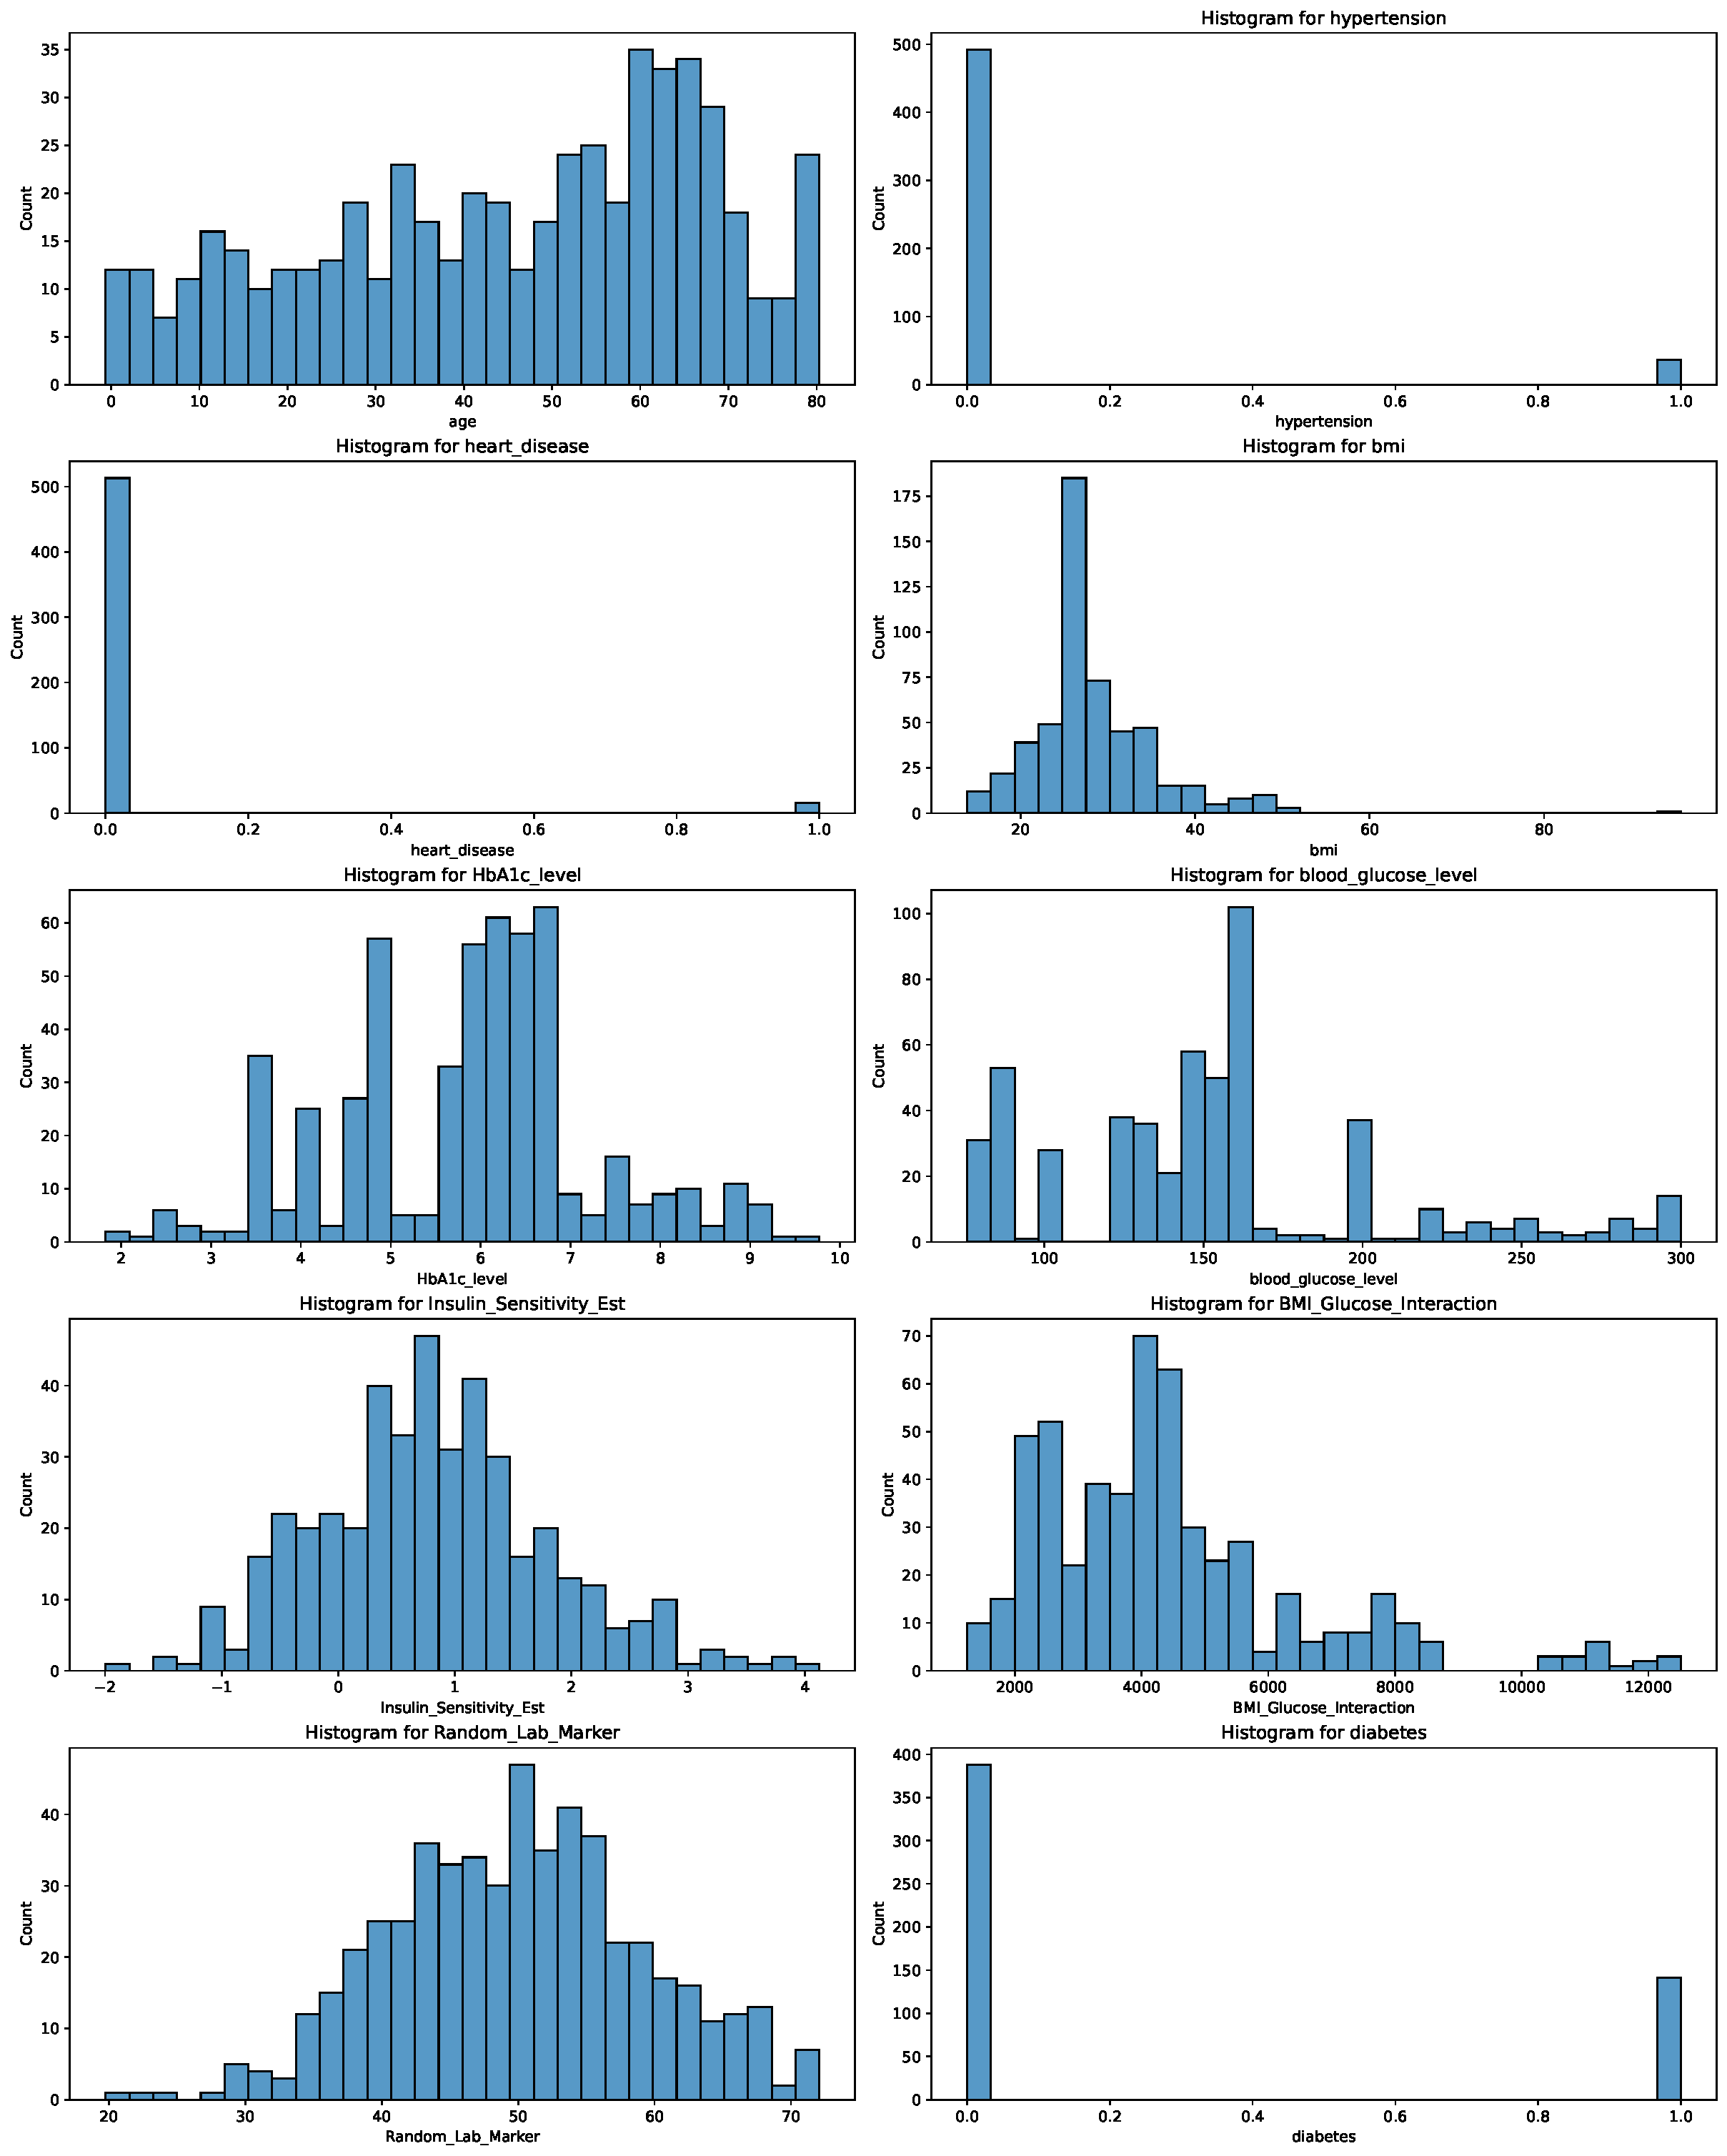
\includegraphics[width=0.45\textwidth]{hist_features.pdf}
    \caption{Istogrammi raffiguranti la distribuzione dei valori di ogni feature.}
    \label{hist}
\end{figure}

\begin{figure}[htbp]
    \centering
    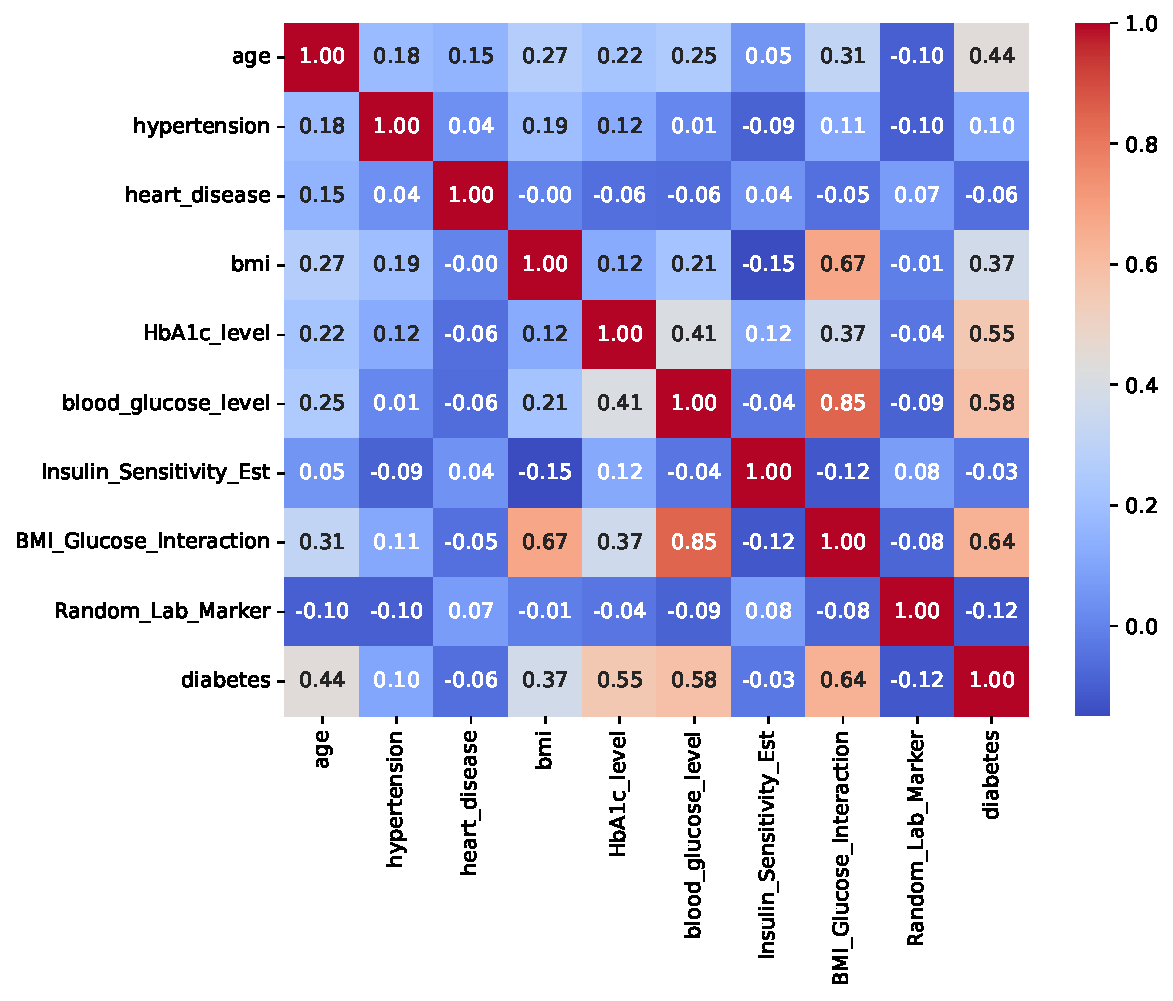
\includegraphics[width=0.40\textwidth]{CorrelationMatrix.pdf}
    \caption{Matrice di correlazione tra le features}
    \label{correlation}
\end{figure}

\section{Metodologia}
%Indicare chiaramente le scelte effettuate per i modelli e una breve descrizione del loro funzionamento e del perchè sono stati usati.
Verificata la qualità dei dati, il dataset è stato partizionato separando le feature dalla variabile target. Si è quindi passati alla selezione degli algoritmi di classificazione, concentrandosi in particolare sui seguenti modelli:
\begin{itemize}
    \item \textbf{Decision Tree}, che permettere di ottenere risultati di facile interpretabilità a basso costo computazionale.
    \item \textbf{Random Forest} un insieme di alberi decisionali costruiti su diversi sottoinsiemi del dataset, che offre maggiore robustezza rispetto al singolo albero, riduce l’overfitting e migliora la precisione della classificazione.
    \item \textbf{Support Vector Machine} un algoritmo efficace per problemi di classificazione binaria, che cerca di trovare l’iperpiano ottimale che separa le due classi massimizzando il margine tra i dati.
    \item \textbf{Multi-layer Perceptron} una rete neurale artificiale in grado di modellare relazioni complesse non lineari tra le variabili. Richiede maggiore potenza computazionale ma può offrire alte prestazioni.
\end{itemize} 

Il tuning degli iperparametri è stato effettuato tramite \texttt{GridSearchCV}, che applica una cross-validation interna per ottimizzare una metrica specifica. La scelta è ricaduta sull'utilizzo di 5 fold e come metrica la F1-Score \footnote{Questa metrica è implementata da SkLearn come descritto nella \href{https://scikit-learn.org/stable/modules/generated/sklearn.metrics.f1_score.html}{loro documentazione}.} scelta per gestire lo sbilanciamento tra le classi, dove altre metriche, come l'accuratezza, risulterebbero poco affidabili e fuorvianti. Il numero di fold è stato determinato sperimentalmente, confrontando le performance su train e test set.
%Si è visto che questo valore era il migliore ed evitava l'overfitting.
Una volta individuati gli iparametri migliori, il modello è stato allenato nuovamente su tutto il dataset di train.

\subsection{Decision Tree}
Sono stati testati diversi iperparametri per il Decision Tree: come misura d’impurità \textit{Gini index} e \textit{Entropy}; profondità massima (10, 20, 50); numero minimo di campioni per split (2, 5, 10) e soglia minima di riduzione dell’impurità (0.001, 0.01, 0.1). La configurazione ottimale è risultata \{Gini, 20, 2, 0.001\}. Dall’albero risultante, riportato nella Figura \ref{tree}, è possibile identificare visualmente le feature che maggiormente influenzano la classificazione, essendo utilizzate come attributi di splitting nei nodi più alti. Come ipotizzato precedentemente, gli attributi \emph{HbA1c\_level} e \emph{blood\_glucose\_level} risultano particolarmente rilevanti, insieme a \emph{age} e \emph{bmi}, presenti anche loro tra i primi nodi di splitting.


\begin{figure} [H]
    \centering
    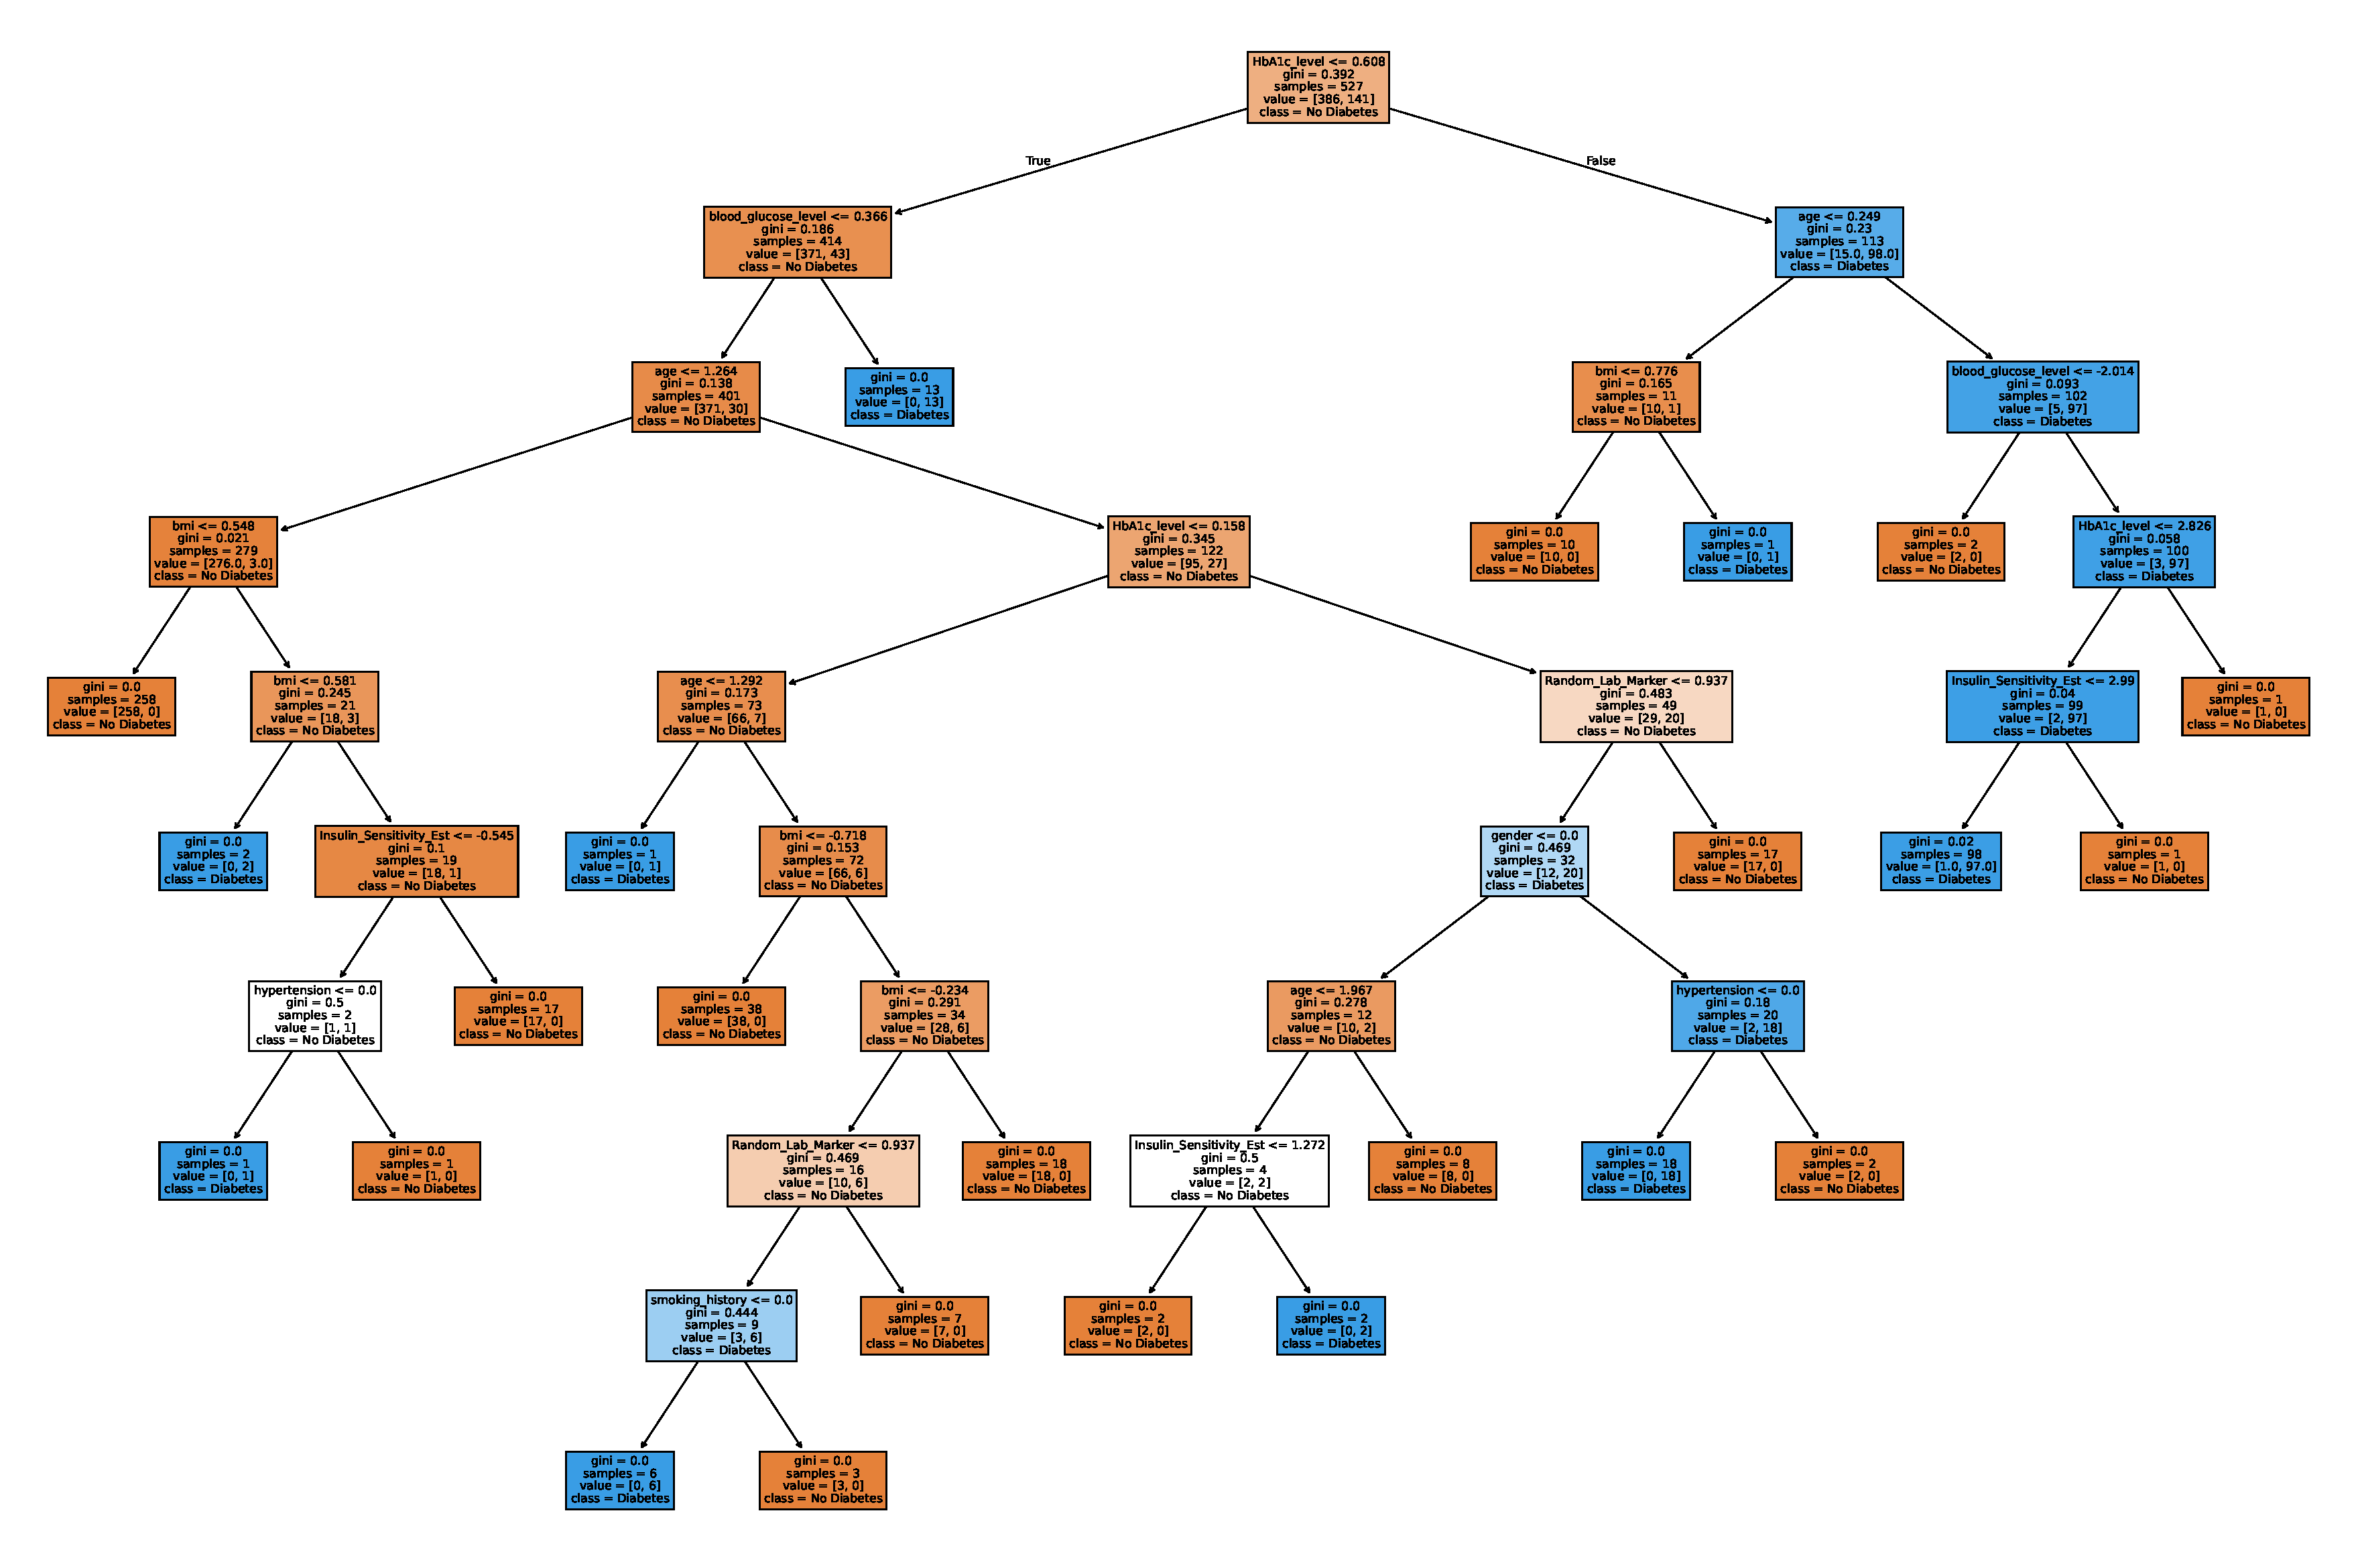
\includegraphics[width=\linewidth]{DecisionTree.pdf}
    \caption{Decision Tree}
    \label{tree}
\end{figure}

\subsection{Random Forest}
Per il Random Forest sono stati testati diversi iperparametri: numero di alberi stimatori (50, 100), profondità massima (10, 20, 50), minimo numero di campioni per split (2, 5, 10) e soglia minima di riduzione dell’impurità (0.01, 0.1, 0). L’ottimizzazione ha individuato come configurazione migliore \{50, 50, 2, 0.0\}.

\subsection{Support vector Machine}
I prinicipali iperparametri del SVM testati sono stati i seguenti: il kernel, che definisce il tipo di confine decisionale (scelto tra lineare, rbf e sigmoid); il parametro C, il coefficiente di regolarizzazione tra 0.01, 0.2, 2, 10; il gamma, che controlla l’influenza dei singoli punti tra i valori auto (che corrisponde a $1 / \text{num\_feature}$), 0.01 e 1/30. La combinazione di parametri che è risultata migliore è \{rbf, 2, auto\}.

\subsection{Multi-layer Perceptron}
Per la grid-search del MLP sono state testate diverse configurazioni di rete, variando numero di layer e neuroni ((15,7,15), (11,15,11), (11,11,11,11,11)), funzioni di attivazione (ReLU, identità), learning rate (costante, adattivo) e solver (\textit{Adam}, \textit{sgd}). Il numero massimo di iterazioni è stato fissato a 3000.
La combinazione migliore è risultata \{ (15, 7, 15), ReLu, learning rate adattativo, solver adam\}.

Il fatto che tra le migliori performance del MLP ve ne sia una ottenuta con funzione di attivazione identitaria (ovvero con una rete lineare) ci ha suggerito che probabilmente una PCA \footnote{PRINCIPAL COMPONENT ANALYSIS: metodo che utilizza la combinazione lineare delle feature e la matrice di covarianza per la ricerca delle direzioni di massima varianza spiegata. Nel dataset considerato, l'85\% della varianza è spiegato da 6 principal component
\begin{figure} [H]
    \centering
    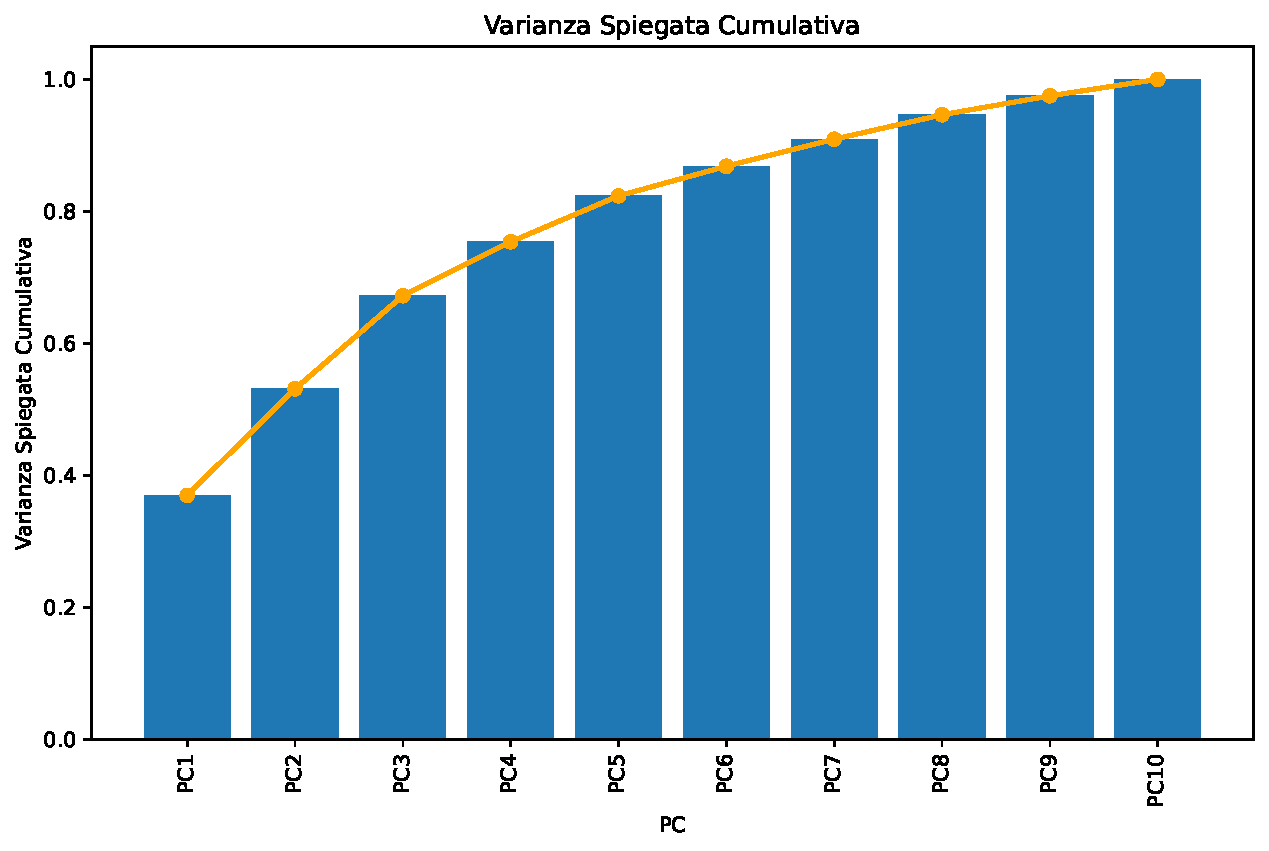
\includegraphics[width=0.3\linewidth]{varianzaSpiegataCumulativa.pdf}
    \caption{\footnotesize Varianza Spiegata Cumulativa }
    \label{varianzaSpiegataCumulativa}
\end{figure}}
applicata sul dataset avrebbe avuto un'alta varianza spiegata anche con poche componenti.


\section{Risultati sperimentali}
%Presentare i risultati ottenuti mettendo in luce forze e debolezze delle varie proposte. Se ritenuto utile riportare anche degli esempi pratici per faciliatere la comprensione. Indicare i parametri usati per i risultati presentati.
Utilizzando i parametri selezionati nella sezione precedente, si riportano di seguito le matrici di confusione dei vari algoritmi sia applicati al dataset di train sia a quello di test. Il confronto tra queste ci ha permesso di valutare se c'è stato overfitting in quanto i dati contenuti nel test non sono mai stati visti in fase di addestramento. 

\begin{table}[H]
\centering
\small
\begin{tabular}{lrr}
\toprule
 & Predicted No Diabetes & Predicted Diabetes \\
\midrule
Actual No Diabetes & 385 & 1 \\
Actual Diabetes & 0 & 141 \\
\bottomrule
\end{tabular}
\caption{Matrice di confusione del dataset di train con DT.}
\label{tab:DT_CF_TRAIN}
\end{table}


\begin{table}[H]
\centering
\small
\begin{tabular}{lrr}
\toprule
 & Predicted No Diabetes & Predicted Diabetes \\
\midrule
Actual No Diabetes & 109 & 1 \\
Actual Diabetes & 3 & 34 \\
\bottomrule
\end{tabular}
\caption{Matrice di confusione del dataset di test con DT.}
\label{tab:DT_CF_TEST}
\end{table}

\begin{table}[H]
\centering
\small
\begin{tabular}{lrr}
\toprule
 & Predicted No Diabetes & Predicted Diabetes \\
\midrule
Actual No Diabetes & 386 & 0 \\
Actual Diabetes & 0 & 141 \\
\bottomrule
\end{tabular}
\caption{Matrice di confusione per il train del RF}
\label{tab:RF_CF_TRAIN}
\end{table}

\begin{table}[H]
\centering
\small
\begin{tabular}{lrr}
\toprule
 & Predicted No Diabetes & Predicted Diabetes \\
\midrule
Actual No Diabetes & 110 & 0 \\
Actual Diabetes & 3 & 34 \\
\bottomrule
\end{tabular}
\caption{Matrice di confusione del test del RF.}
\label{tab:RF_CF_TEST}
\end{table}
Nelle tabelle \ref{tab:DT_CF_TRAIN} e \ref{tab:DT_CF_TEST} relative al Decision Tree si osserva un lieve overfitting, evidenziato da un numero inferiore di errori sul training set. Lo stesso comportamento emerge per il Random Forest, che, essendo un insieme di alberi decisionali, ottiene prestazioni leggermente migliori.

\begin{table}[H]
\centering
\small
\begin{tabular}{lrr}
\toprule
 & Predicted No Diabetes & Predicted Diabetes \\
\midrule
Actual No Diabetes & 382 & 4 \\
Actual Diabetes & 11 & 130 \\
\bottomrule
\end{tabular}
\caption{Matrice di confusione del train del SVM.}
\label{tab:SVM_CF_TRAIN}
\end{table}

\begin{table}[H]
\centering
\small
\begin{tabular}{lrr}
\toprule
 & Predicted No Diabetes & Predicted Diabetes \\
\midrule
Actual No Diabetes & 108 & 2 \\
Actual Diabetes & 5 & 32 \\
\bottomrule
\end{tabular}
\caption{Matrice di confusione del test del SVM.}
\label{tab:SVM_CF_TEST}
\end{table}
Le matrici di confusione dell’SVM (Tabelle \ref{tab:SVM_CF_TRAIN} e \ref{tab:SVM_CF_TEST}) mostrano prestazioni inferiori rispetto ai modelli ad albero, probabilmente a causa del numero ridotto di dati e della difficoltà del modello nel catturare relazioni complesse, anche con kernel RBF (Radial Basis Function Kernel). Un’eventuale soluzione è proiettare le feature in uno spazio più adatto alla separazione lineare.

\begin{table}[H]
\centering
\small
\begin{tabular}{lrr}
\toprule
 & Predicted No Diabetes & Predicted Diabetes \\
\midrule
Actual No Diabetes & 385 & 1 \\
Actual Diabetes & 2 & 139 \\
\bottomrule
\end{tabular}
\caption{Matrice di confusione del train del MLP.}
\label{tab:MLP_CF_TRAIN}
\end{table}

\begin{table}[H]
\centering
\small
\begin{tabular}{lrr}
\toprule
 & Predicted No Diabetes & Predicted Diabetes \\
\midrule
Actual No Diabetes & 109 & 1 \\
Actual Diabetes & 4 & 33 \\
\bottomrule
\end{tabular}
\caption{Matrice di confusione del test del MLP.}
\label{tab:MLP_CF_TEST}
\end{table}


Nel contesto di questo studio, sono stati confrontati, inoltre, i quattro algoritmi usando le seguenti misure per la prestazione di ciascun modello : Precision (p), Recall (r) e F1-score (F1) per ciascuna delle due classi: "0" (nessuna malattia) e "1" (presenza di malattia).
\begin{table}[H]
\centering
\small
\begin{tabular}{l|rrr|rrr|rrr|rrr}
\toprule
\textbf{Model} & \multicolumn{3}{c|}{\textbf{Class 0}} & \multicolumn{3}{c|}{\textbf{Class 1}} \\
\cmidrule(r){2-4} \cmidrule(r){5-7}
 & \textbf{p} & \textbf{r} & \textbf{F1} & \textbf{p} & \textbf{r} & \textbf{F1} \\
\midrule
\textbf{DT} & 0.97 & 0.99 & 0.98 & 0.97 & 0.92 & 0.94 \\
\textbf{RF} & 0.97 & 1.00 & 0.99 & 1.00 & 0.92 & 0.96 \\
\textbf{SVM} & 0.96 & 0.98 & 0.97 & 0.94 & 0.86 & 0.90 \\
\textbf{MLP} & 0.96 & 0.99 & 0.98 & 0.97 & 0.89 & 0.93 \\
\bottomrule
\end{tabular}
\caption{Confronto tra RF, DT, MLP e SVM con le metriche di precision, recall e F1-score per le classi 0 e 1 sul test.}

\label{tab:classification_report_comparison_1}
\end{table}

Il Random Forest risulta il modello migliore, probabilmente per la relativa semplicità del problema, offrendo anche una maggior robustezza rispetto al singolo Decision Tree. In tutti i modelli, la classe 1 presenta performance inferiori rispetto alla classe 0, a causa dello sbilanciamento nel dataset di training.

Nel Random Forest, per la classe dei pazienti malati si ottiene una precisione pari a 1 e un recall pari a 0.92 ciò significa che tutti i casi predetti come malati sono corretti, ma alcuni pazienti malati non vengono riconosciuti, un aspetto critico poiché sarebbe preferibile evitare di trascurare casi potenzialmente gravi.

L’SVM mostra performance più equilibrate, con precisione 0.94 e recall 0.86 sulla classe 1, risultando abbastanza affidabile nel rilevare il diabete, anche se tende a non identificare tutti i positivi. Dal punto di vista interpretativo, l'SVM sarebbe più interpretabile del MLP solo con kernel lineare e numero di feature molto basso (2 o 3). In generale, invece, si comporta come una black box.
%l’SVM è più trasparente rispetto al MLP, soprattutto con kernel lineare, ma meno rispetto ai modelli basati su alberi decisionali poiché l'SVM divide i dati secondo degli iperpiani, non necessariamente lineari, in dimensioni alte.


%il modello è molto cauto nel classificare un caso come "malato", ma quando lo fa, non sbaglia mai
 Il MLP mostra performance leggermente inferiori rispetto agli alberi decisionali, commettendo più errori  soprattutto nel riconoscimento dei pazienti malati. Ciò può essere dovuto all’esiguo numero di record, dato che le reti neurali, pur essendo tra i modelli più accurati, richiedono generalmente un maggior quantitativo di dati. 
 Inoltre, a differenza di modelli interpretabili come Decision Tree e Random Forest, il MLP è un modello “black-box”, offrendo scarsa trasparenza nelle decisioni e rendendo più difficile l’interpretazione dei risultati.


Come già evidenziato, una criticità del dataset è il forte sbilanciamento tra le due classi di risposta. Per affrontarlo, si possono utilizzare tecniche di \textbf{upsampling} o \textbf{downsampling}, ovvero rispettivamente l’inserimento di record per la classe minoritaria (diabetici) o la riduzione di quelli per la classe maggioritaria (non diabetici), preservando la rappresentatività della popolazione originale.
Esperimenti empirici\footnote{Gli esperimenti di upsampling/downsampling sono stati condotti tramite funzioni della libreria \texttt{Imbalanced-Learn} in Python.} mostrano che i metodi di downsampling tendono a peggiorare le performance, poiché riducono eccessivamente il numero di record, favorendo l’overfitting nei modelli. L’utilizzo della tecnica di upsampling \texttt{SMOTE} (Synthetic Minority Over-sampling Technique)\footnote{\texttt{SMOTE} genera nuovi campioni sintetici della classe minoritaria interpolando tra istanze vicine.} ha migliorato le prestazioni del SVM, tuttavia ha avuto un effetto negativo sulla capacità predittiva dell’albero decisionale, che risulta più sensibile alla presenza di dati sintetici. Un'analisi più esaustiva andrebbe fatta comparando le performance di varie tecniche di bilanciamento di un dataset.


\section{Conclusioni}
%Indicare come è possibile sfruttare i dati per un applicazione di business.
Gli algoritmi di classificazione presentati possono essere molto preziosi non solo nel settore medico, per avere diagnosi più affidabili e possibilmente precoci contenendo le spese mediche, ma anche nel settore assicurativo. Infatti, grazie ad essi, le compagnie assicurative possono valutare con maggiore precisione il rischio di diabete nei clienti, definendo polizze assicurative personalizzate. 

\section{Contributi}
%Indicare i contributi personali.
Il lavoro è stato svolto insieme da tutti i componenti del gruppo, quindi ognuno ha lavorato in egual modo a tutte le parti del progetto. $\heartsuit$


\end{document}


